Let define, respectively, equations \eqref{eq:Xg} and \eqref{eq:Xh} with the functions $g(k_t, N_t^y, K_t, \eta_t; \phi, \sigma)$ and $h(k_t ; \gamma, \phi, \sigma)$ such as:
\begin{align*}
	g(k_t, N_t^y, K_t, \eta_t; \phi, \sigma) &= \ln\left( \frac{ \frac{N_t^y}{K_t} k_t - 1 } { \frac{\phi}{1-\phi} k_t^{\frac{\sigma-1}{\sigma}} \eta_t - 1 }\right) \\
	h(k_t ; \gamma, \phi, \sigma) &= \left( \sigma + \frac{1-\phi}{\phi} \frac{1-\gamma(1-\sigma)}{\gamma} k_t^{\frac{1-\sigma}{\sigma}} \right)^{-1}
\end{align*}

% \subsection*{A.1 Analysis of the $g$ function}

Due to the logarithm, we have two vertical asymptotes depending on whether the numerator or the denominator within the logarithm is equal to zero. The first vertical asymptote is the one associated to the numerator $k_1 = \frac{K_t}{N_t^y}$ and the second vertical asymptote is associated to the denominator $k_2 = \left(\frac{1-\phi}{\phi} \frac{1}{\eta_t}\right)^{\frac{\sigma}{\sigma-1}}$. Rewriting the $g$ function with these vertical asymptotes, I have:
\begin{equation*}
g(k_t, k_1, k_2; \sigma) = \ln\left( \frac{\frac{k_t}{k_1}-1}{\left(\frac{k_t}{k_2}\right)^{\frac{\sigma - 1}{\sigma}} - 1} \right)
\end{equation*}
This function has four different shapes according to the value of $\sigma$ and both vertical asymptotes ($k_1$ and $k_2$). Figure \ref{fig:g_shape} plots these shapes.
\begin{figure}[tb]
	\begin{subfigure}[b]{0.5\linewidth}
		\centering
		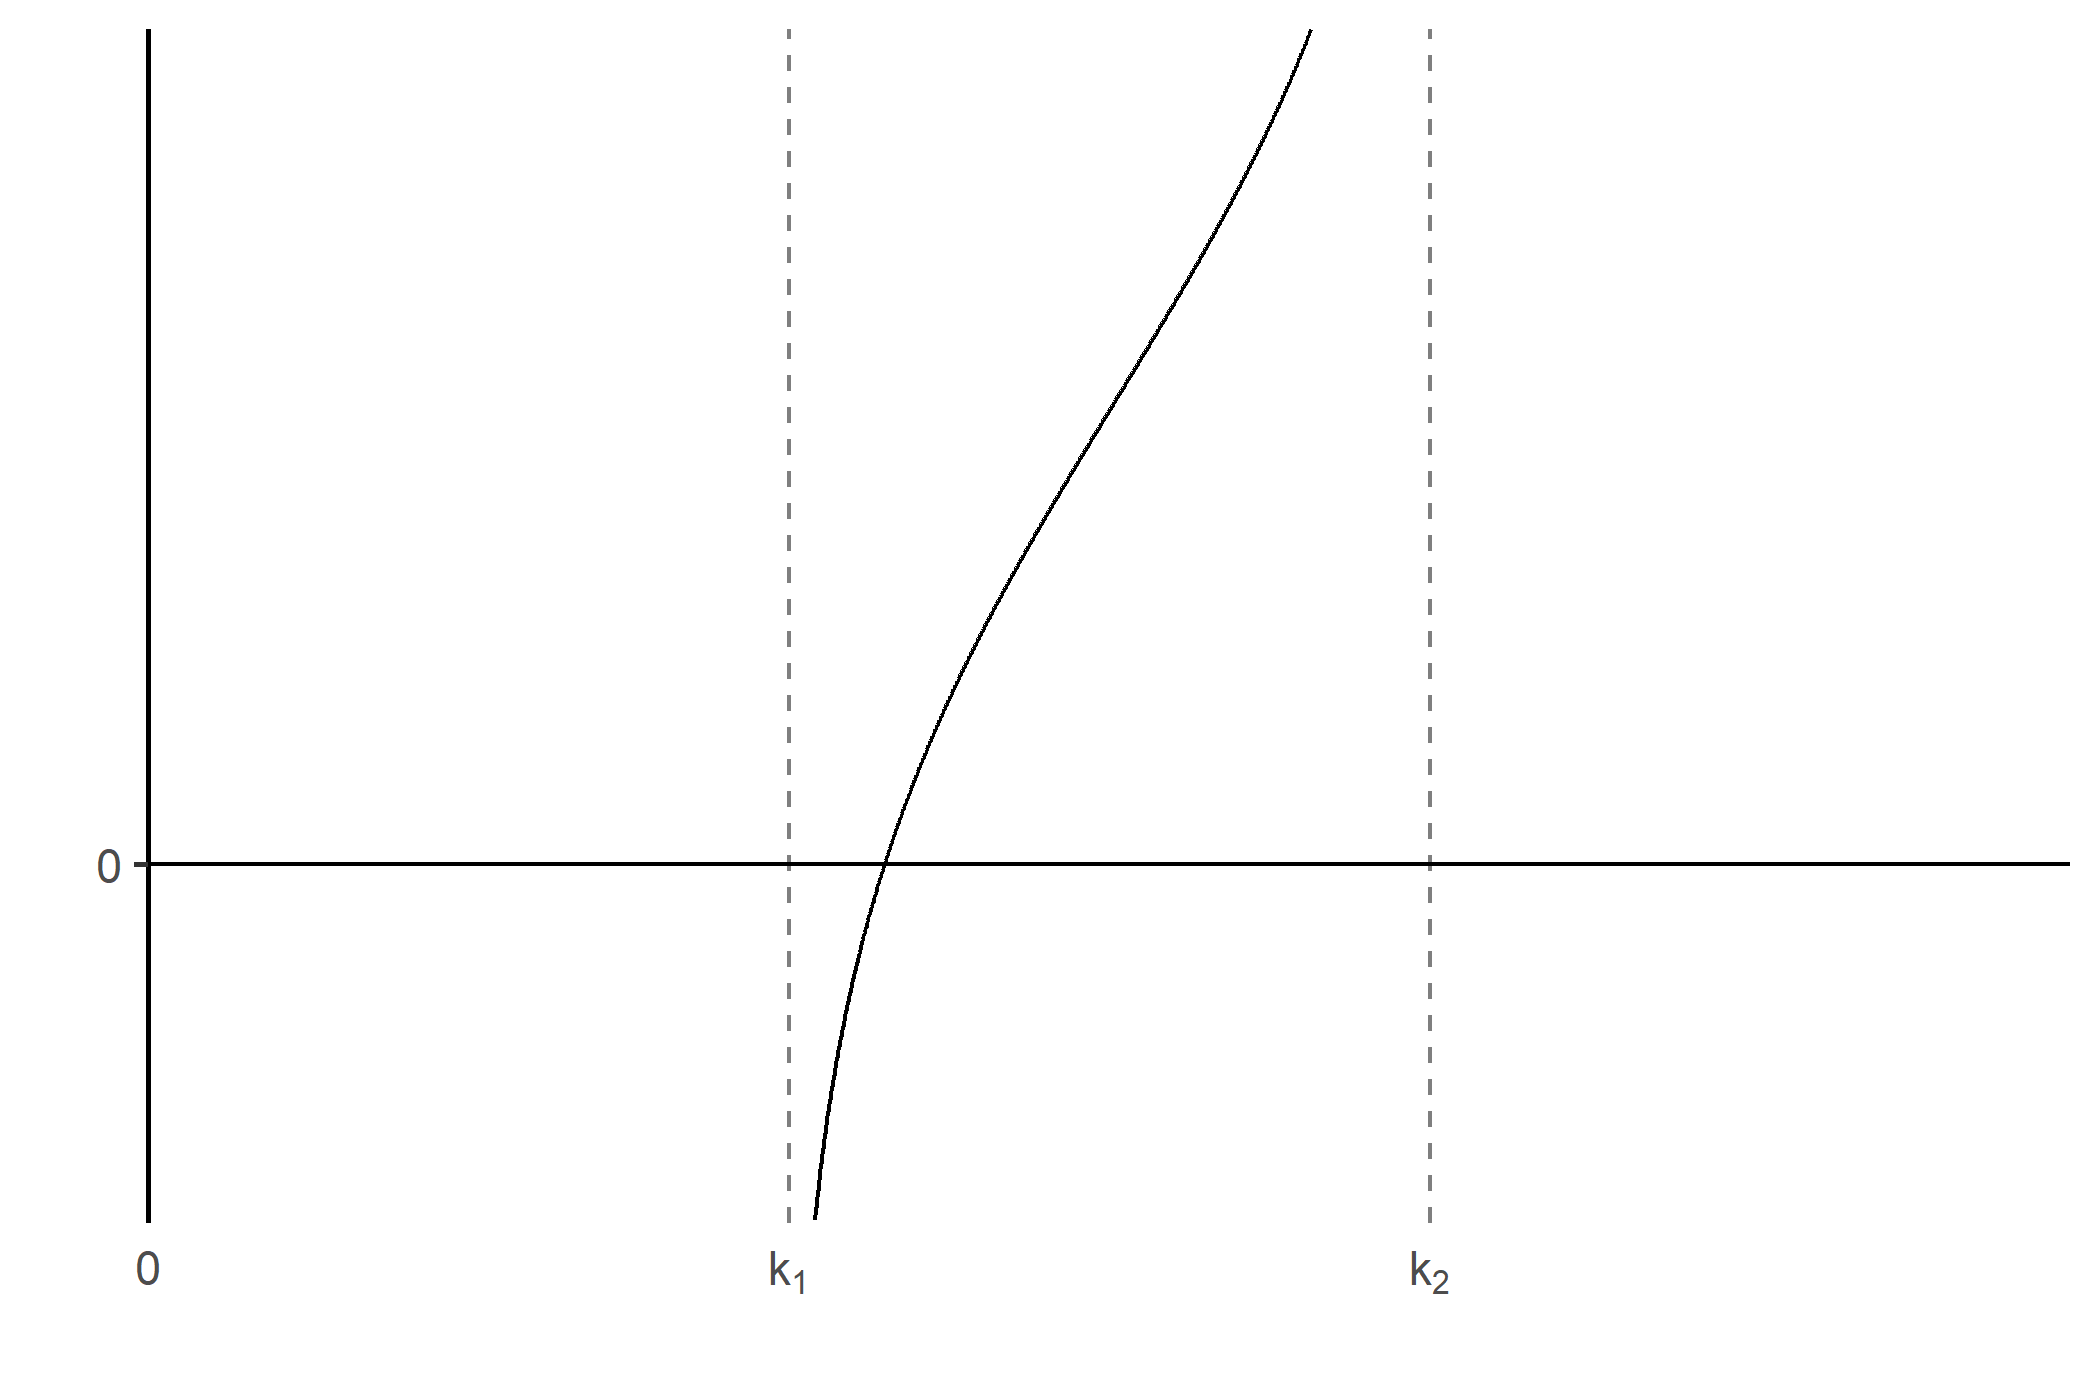
\includegraphics[width=1\linewidth]{../result/appendix_A/function_g/graph_a.png} 
		\caption{$\sigma < 1$, $k_1 < k_2$} 
		\label{fig:g_shape_a}
	\end{subfigure}
	\begin{subfigure}[b]{0.5\linewidth}
		\centering
		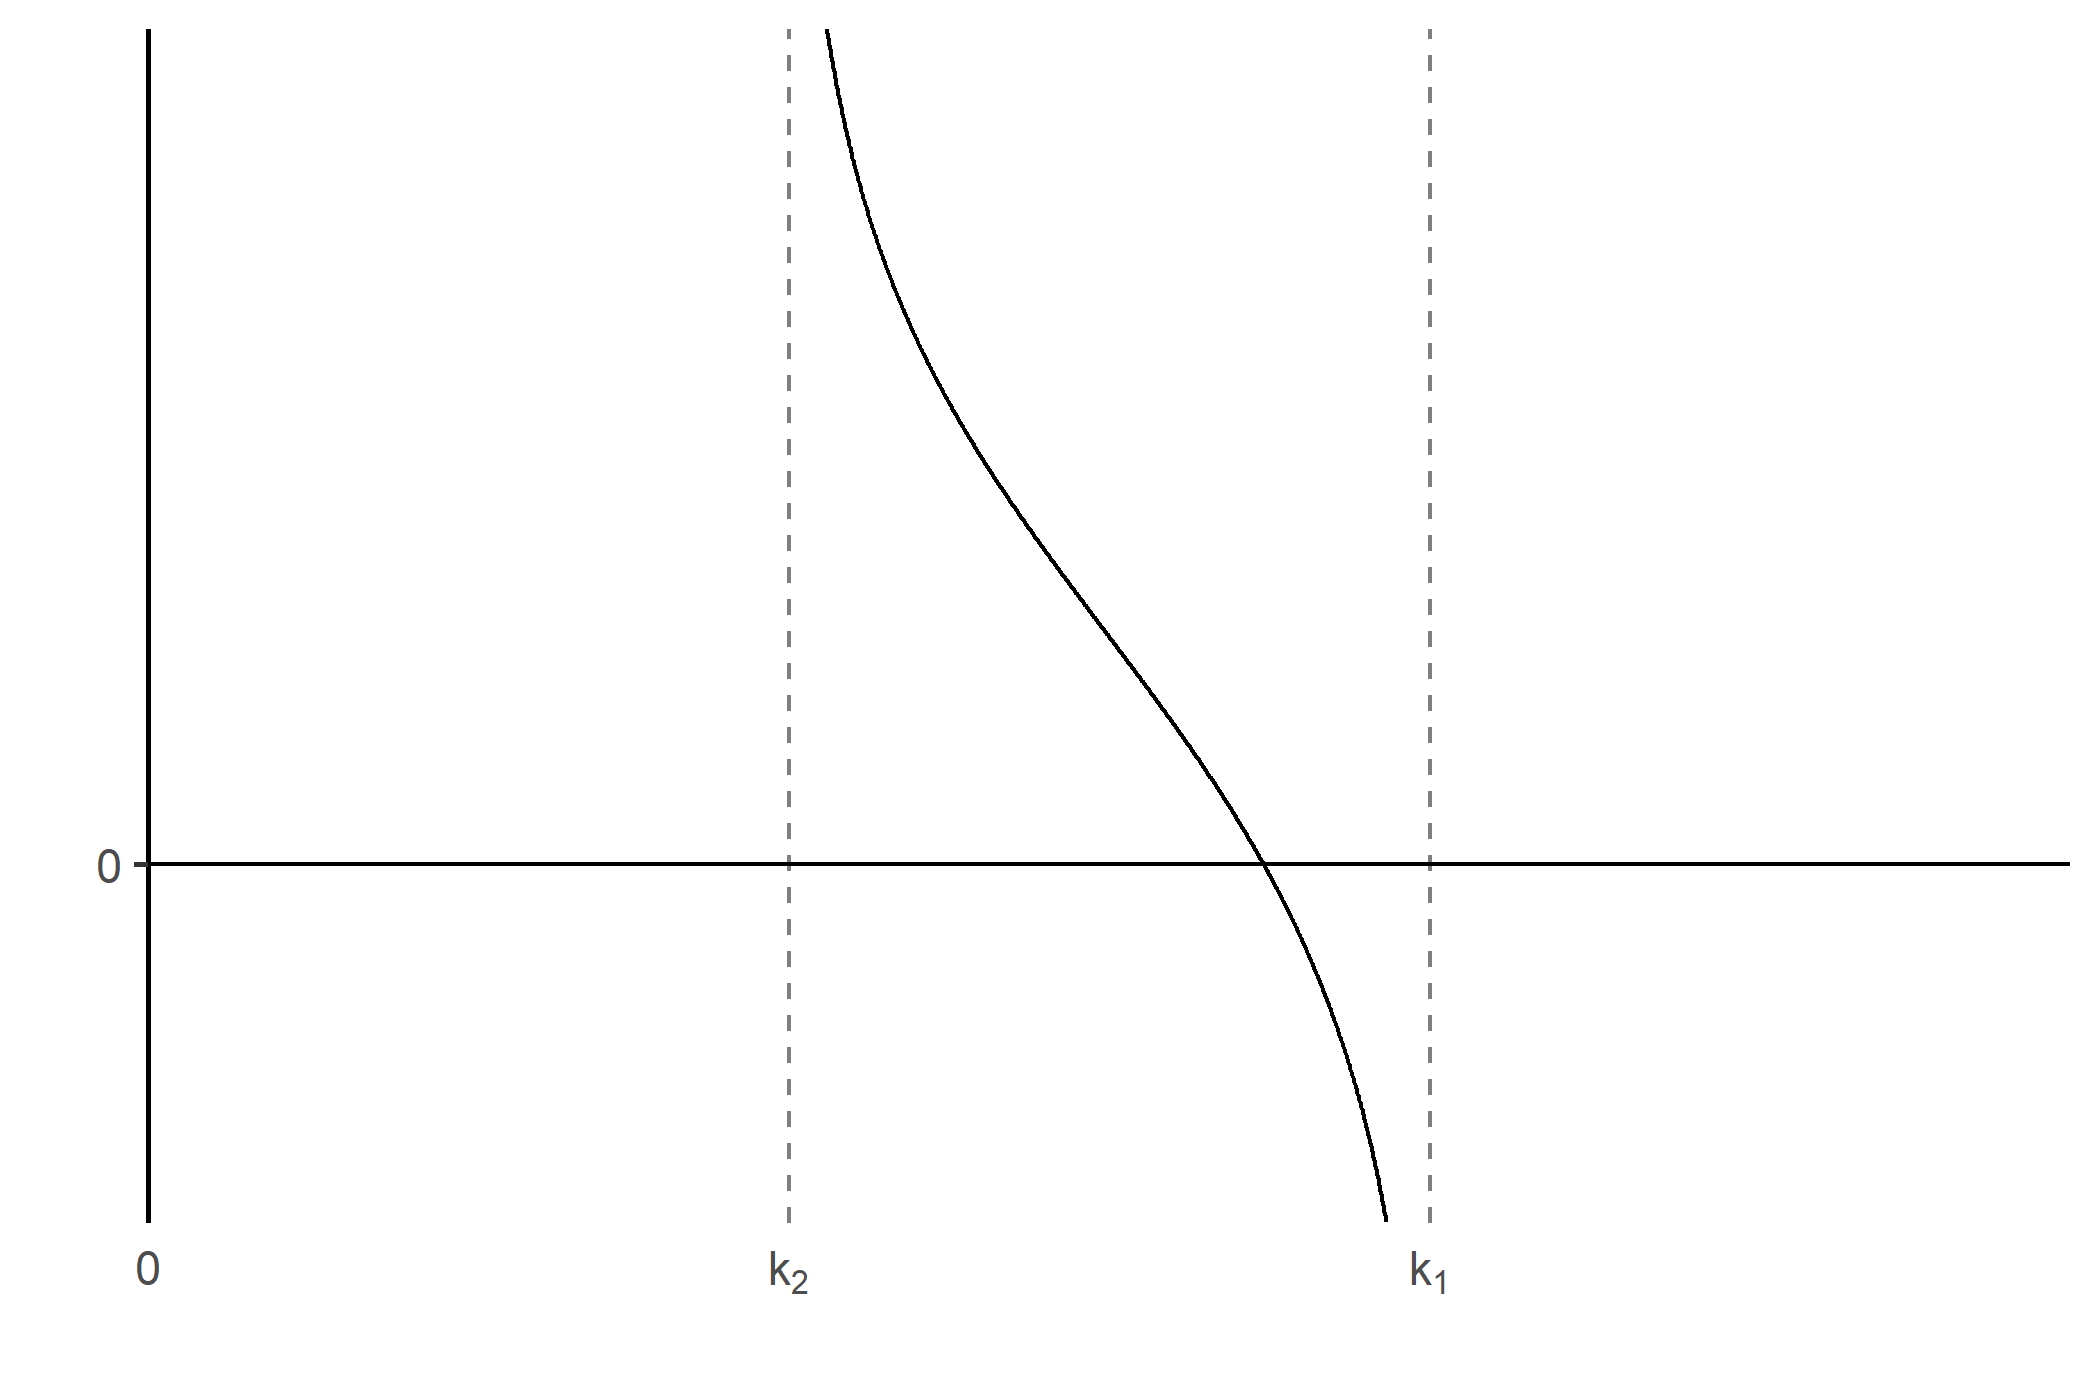
\includegraphics[width=1\linewidth]{../result/appendix_A/function_g/graph_b.png} 
		\caption{$ \sigma < 1$, $k_1 > k_2$}
		\label{fig:g_shape_b}
	\end{subfigure}
	%%%
	\begin{subfigure}[b]{0.5\linewidth}
		\centering
		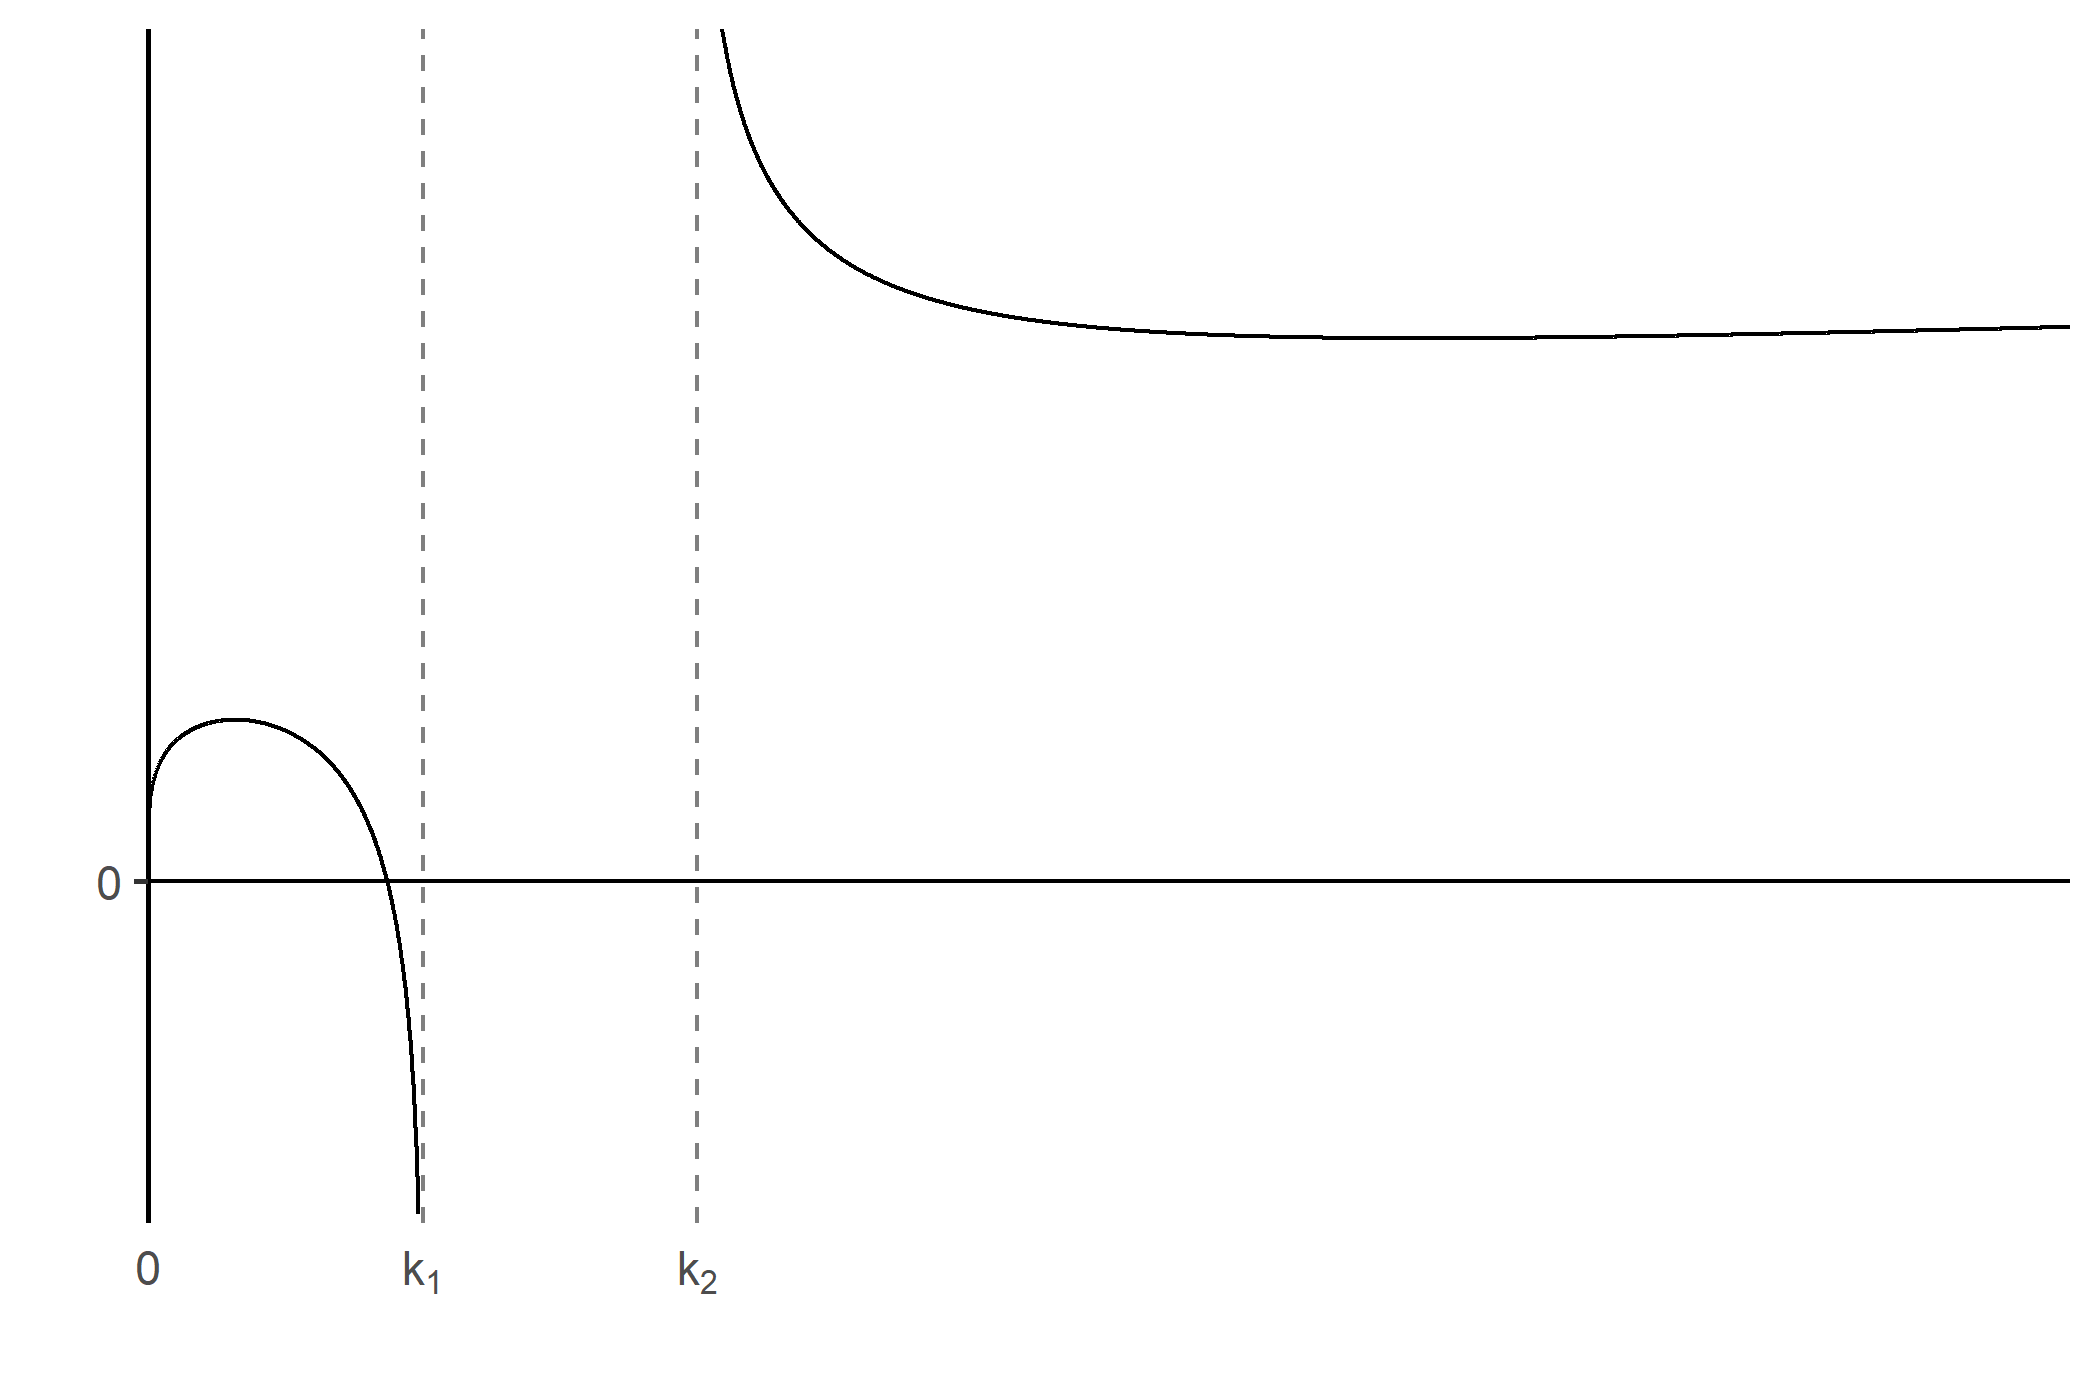
\includegraphics[width=1\linewidth]{../result/appendix_A/function_g/graph_c.png} 
		\caption{$\sigma > 1$, $k_1 < k_2$}
		\label{fig:g_shape_c}
	\end{subfigure}
	\begin{subfigure}[b]{0.5\linewidth}
		\centering
		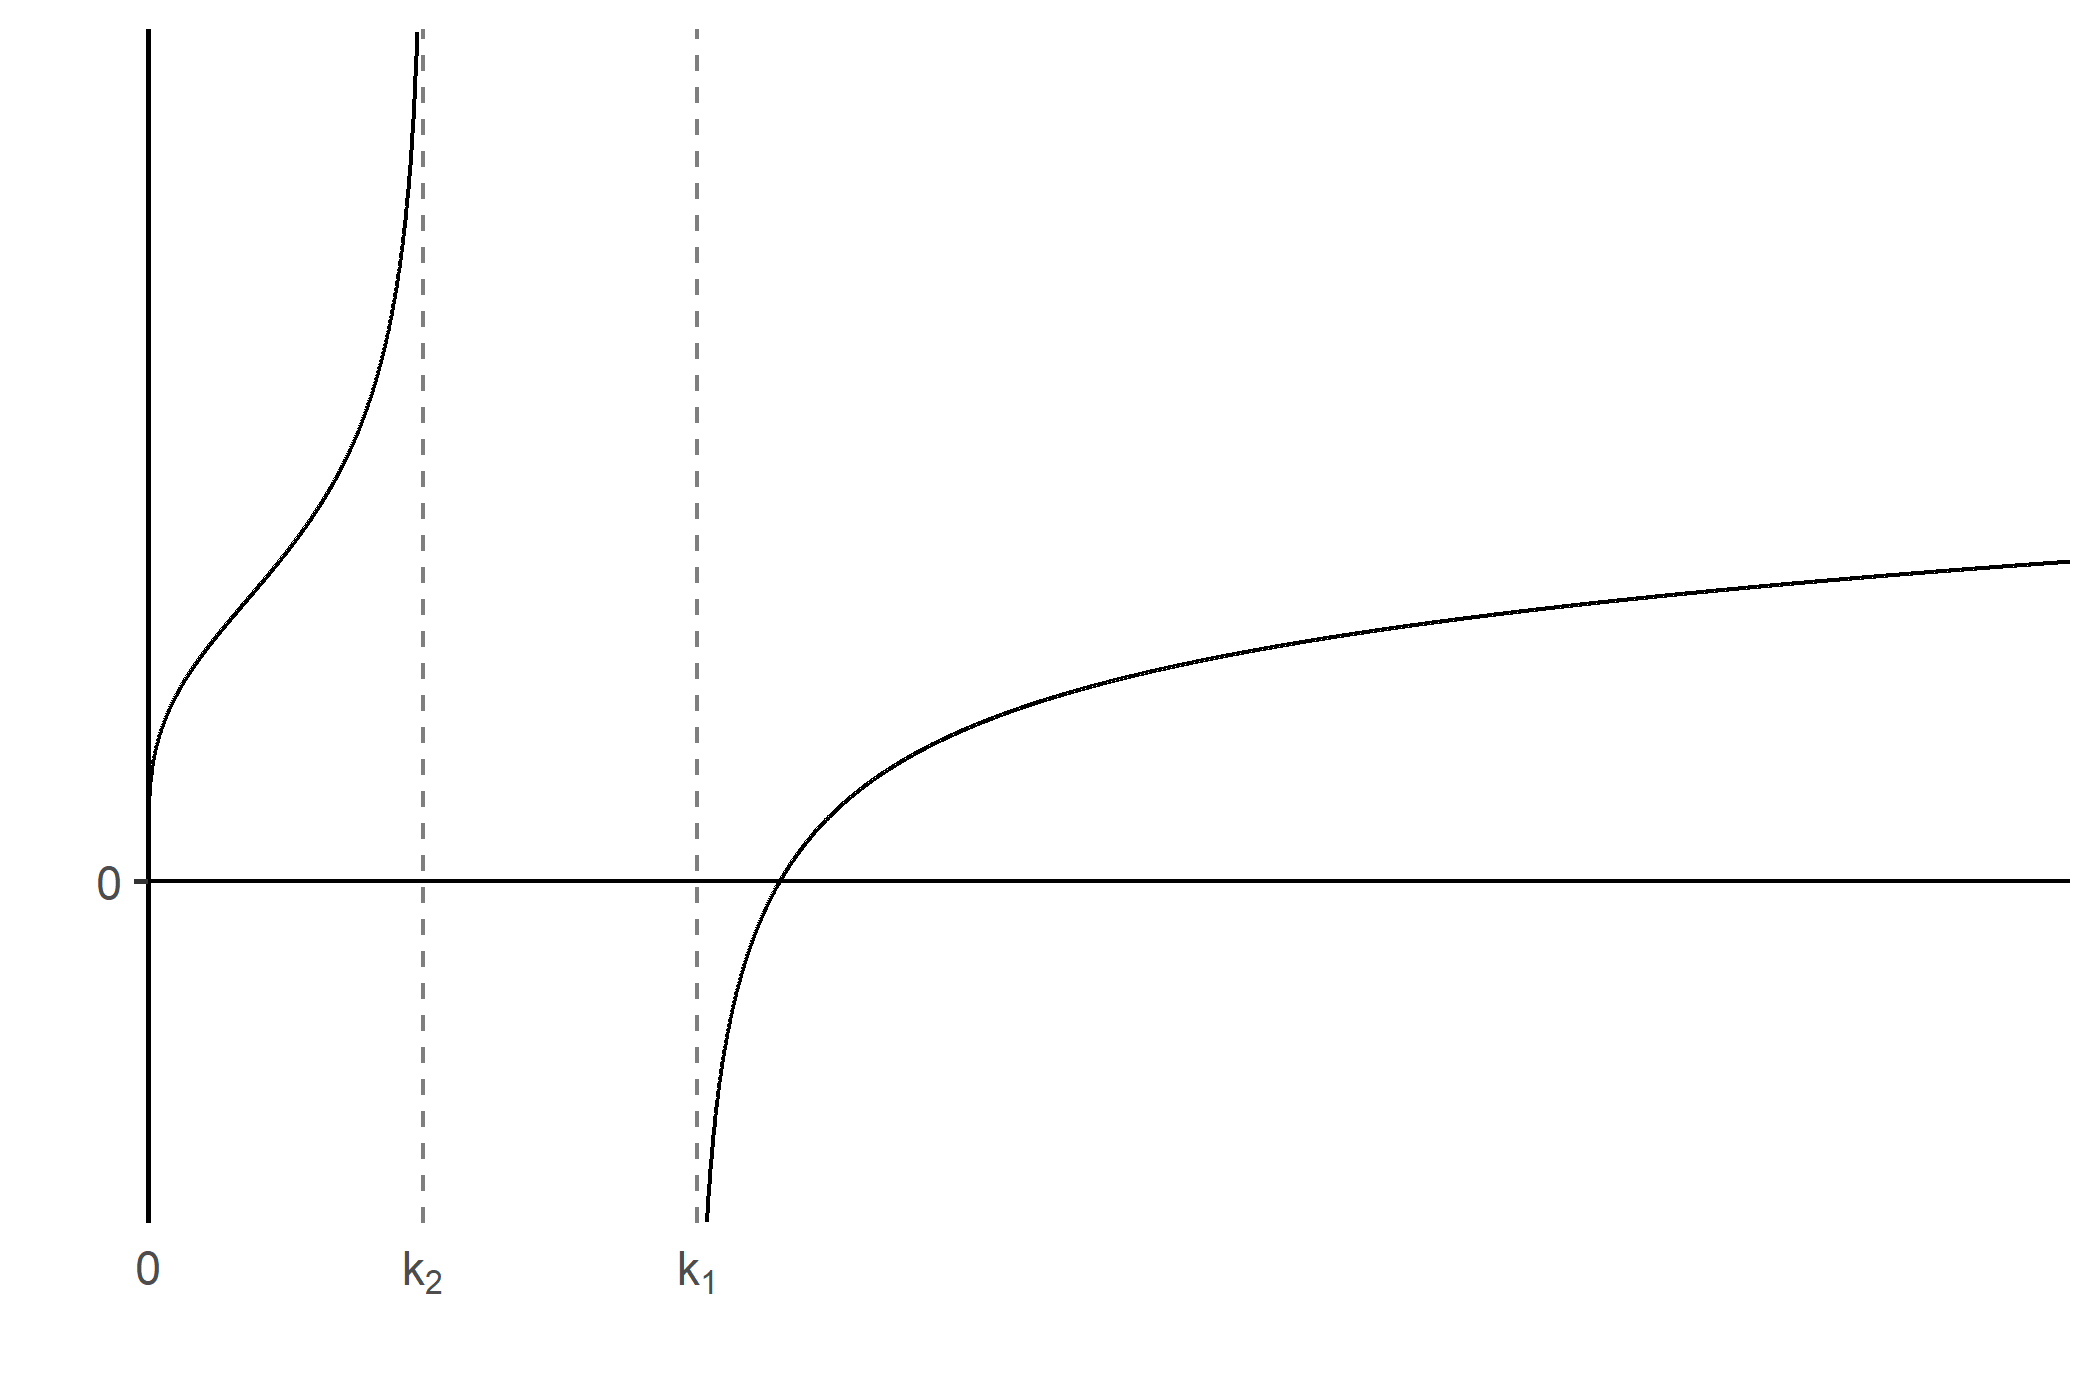
\includegraphics[width=1\linewidth]{../result/appendix_A/function_g/graph_d.png}
		\caption{$\sigma > 1$, $k_1 > k_2$}
		\label{fig:g_shape_d}
	\end{subfigure} 
	\caption{Different possible shapes of the $g$ function, according to the value of $\sigma, k_1, k_2$.}
	\label{fig:g_shape}
	\vspace{.5ex}
	\hrule
	\vspace{-4ex}
	\justify\singlespacing\footnotesize The x-axis corresponds to $k_t$. The function graphs are drawn using numerical computation with the following set of parameters for each case:\\
	(a) $\sigma = 0.8$, $k_1 = 1$, $k_2 = 2$ ; \hspace{2ex}(b) $\sigma = 0.8$, $k_1 = 2$, $k_2 = 1$ ; \\(c) $\sigma = 1.2$, $k_1 = 1$, $k_2 = 2$ ; \hspace{2ex}(d) $\sigma = 1.2$, $k_1 = 2$, $k_2 = 1$.
\end{figure}
The $h$ function has three different shapes according to the value of $\sigma$. Figure \ref{fig:h_shape} plots these shapes.
\begin{figure}[tb]
	\begin{subfigure}[t]{0.32\linewidth}
		\centering
		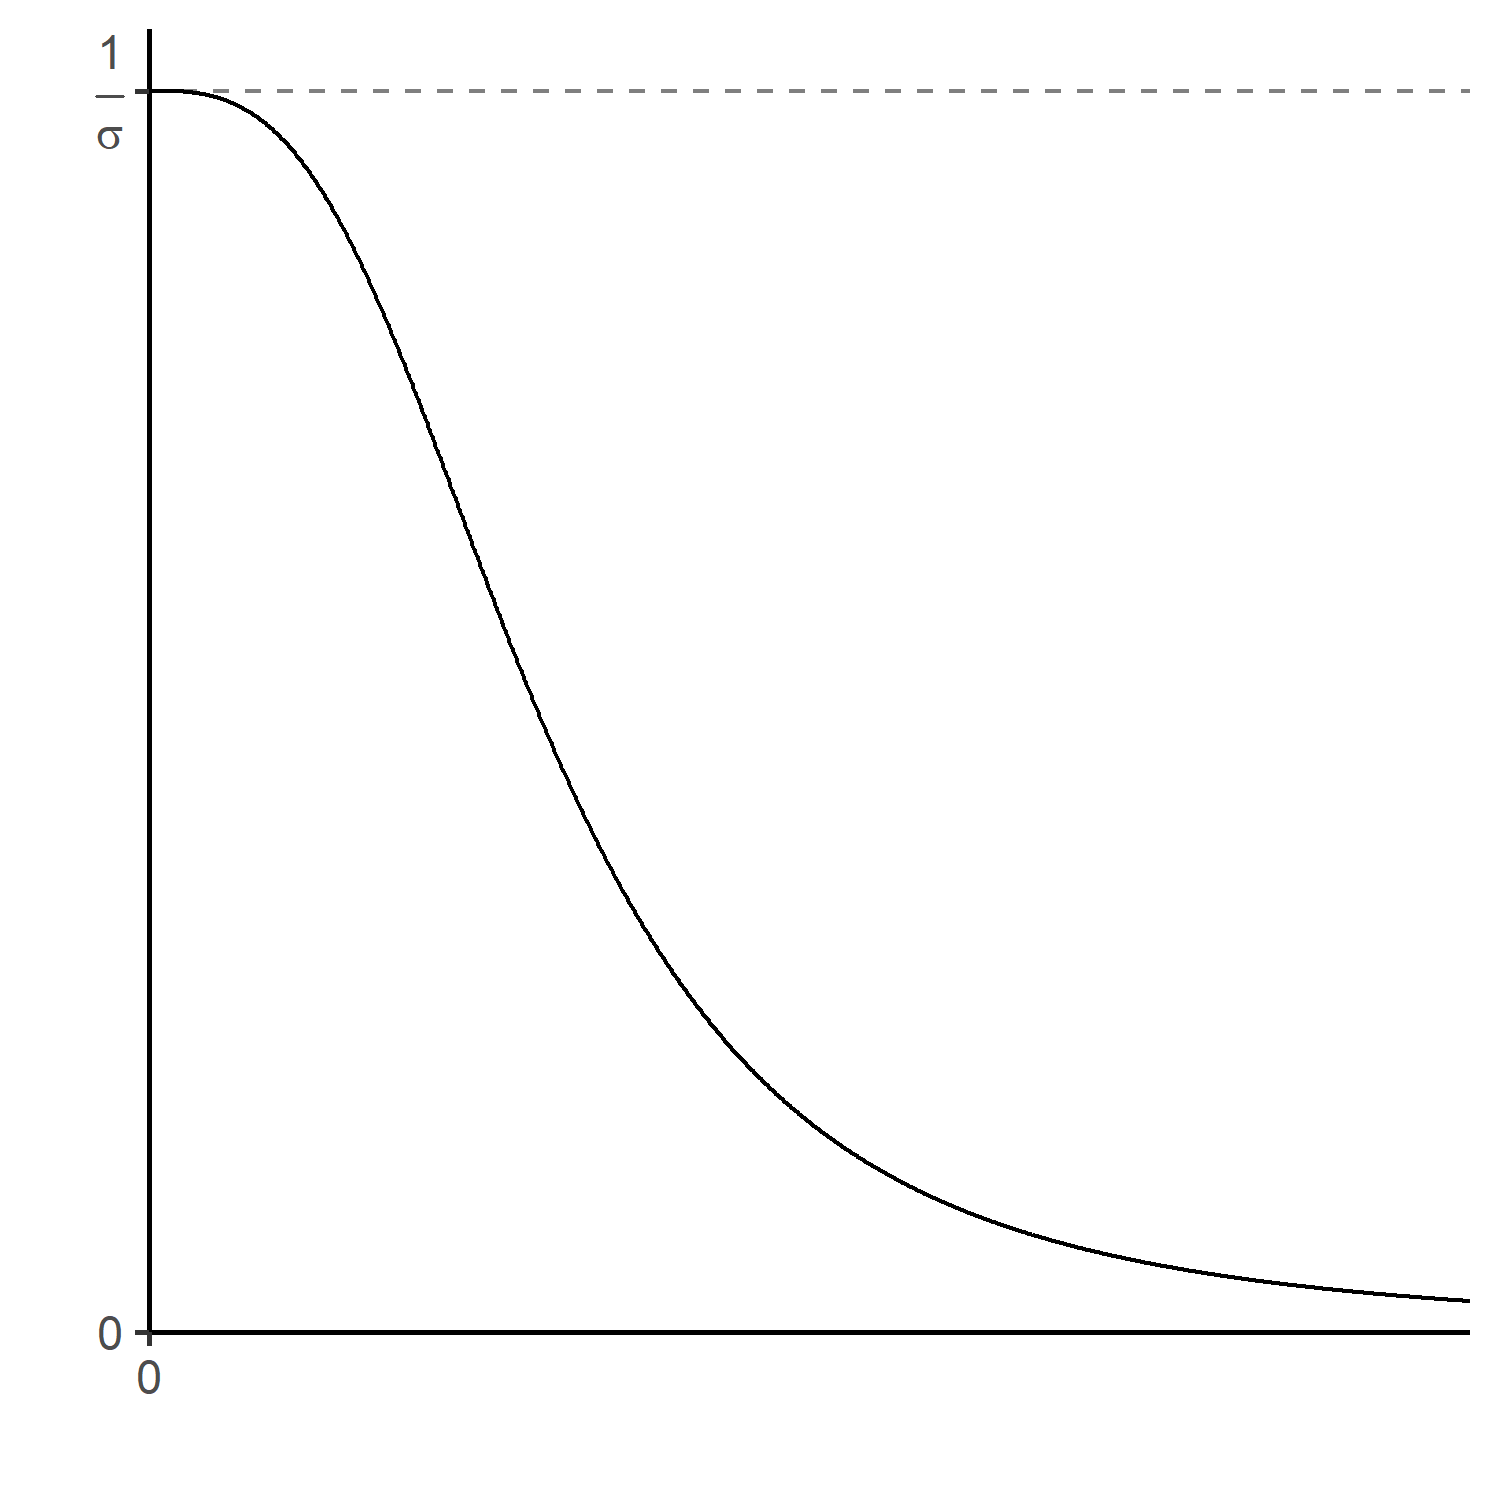
\includegraphics[width=1\linewidth]{../result/appendix_A/function_h/graph_1.png} 
		\caption{$\sigma \leq 0.5$} 
		\label{fig:h_shape_1} 
	\end{subfigure}
	%%%
	\begin{subfigure}[t]{0.32\linewidth}
		\centering
		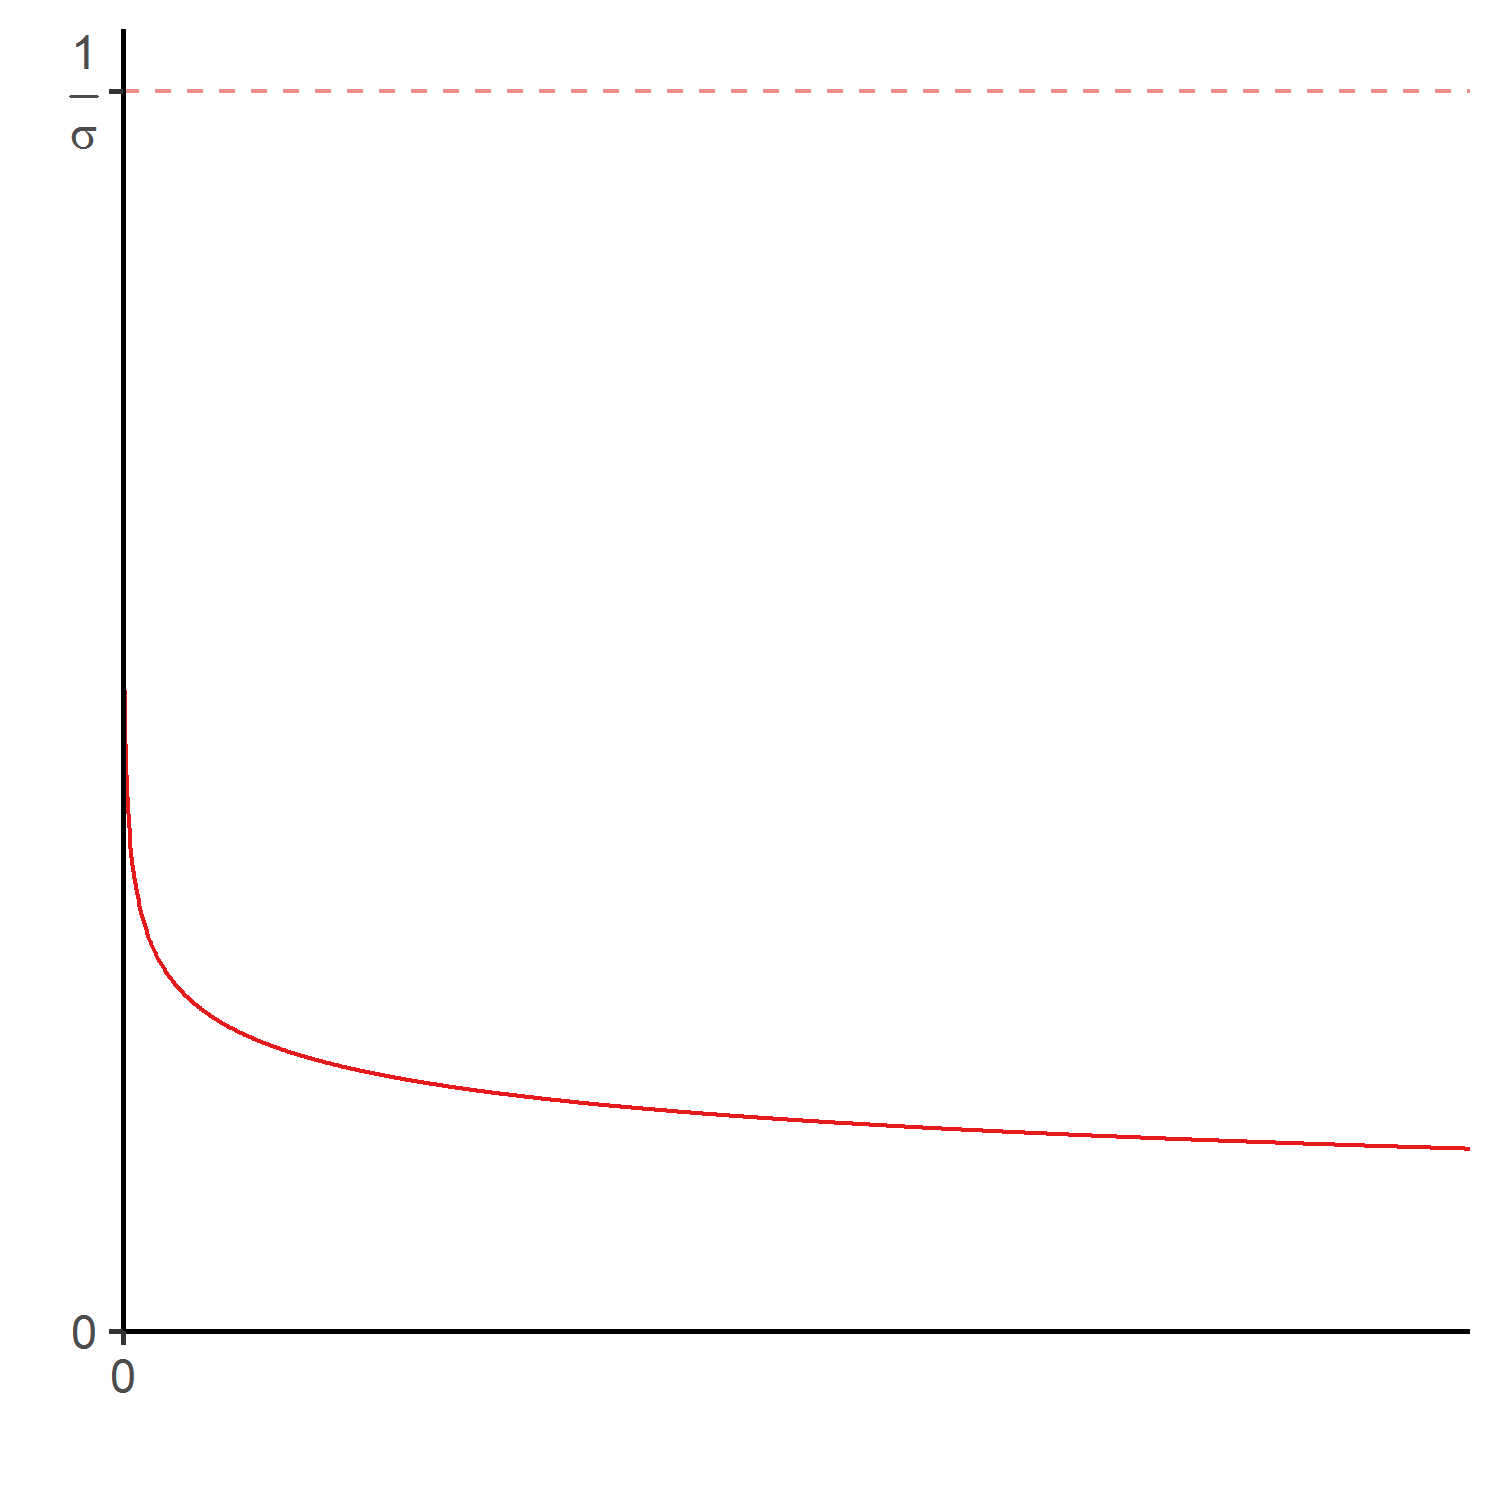
\includegraphics[width=1\linewidth]{../result/appendix_A/function_h/graph_2.png} 
		\caption{$\sigma \in \left(0.5, 1\right)$} 
		\label{fig:h_shape_2} 
	\end{subfigure}
	%%%
	\begin{subfigure}[t]{0.32\linewidth}
		\centering
		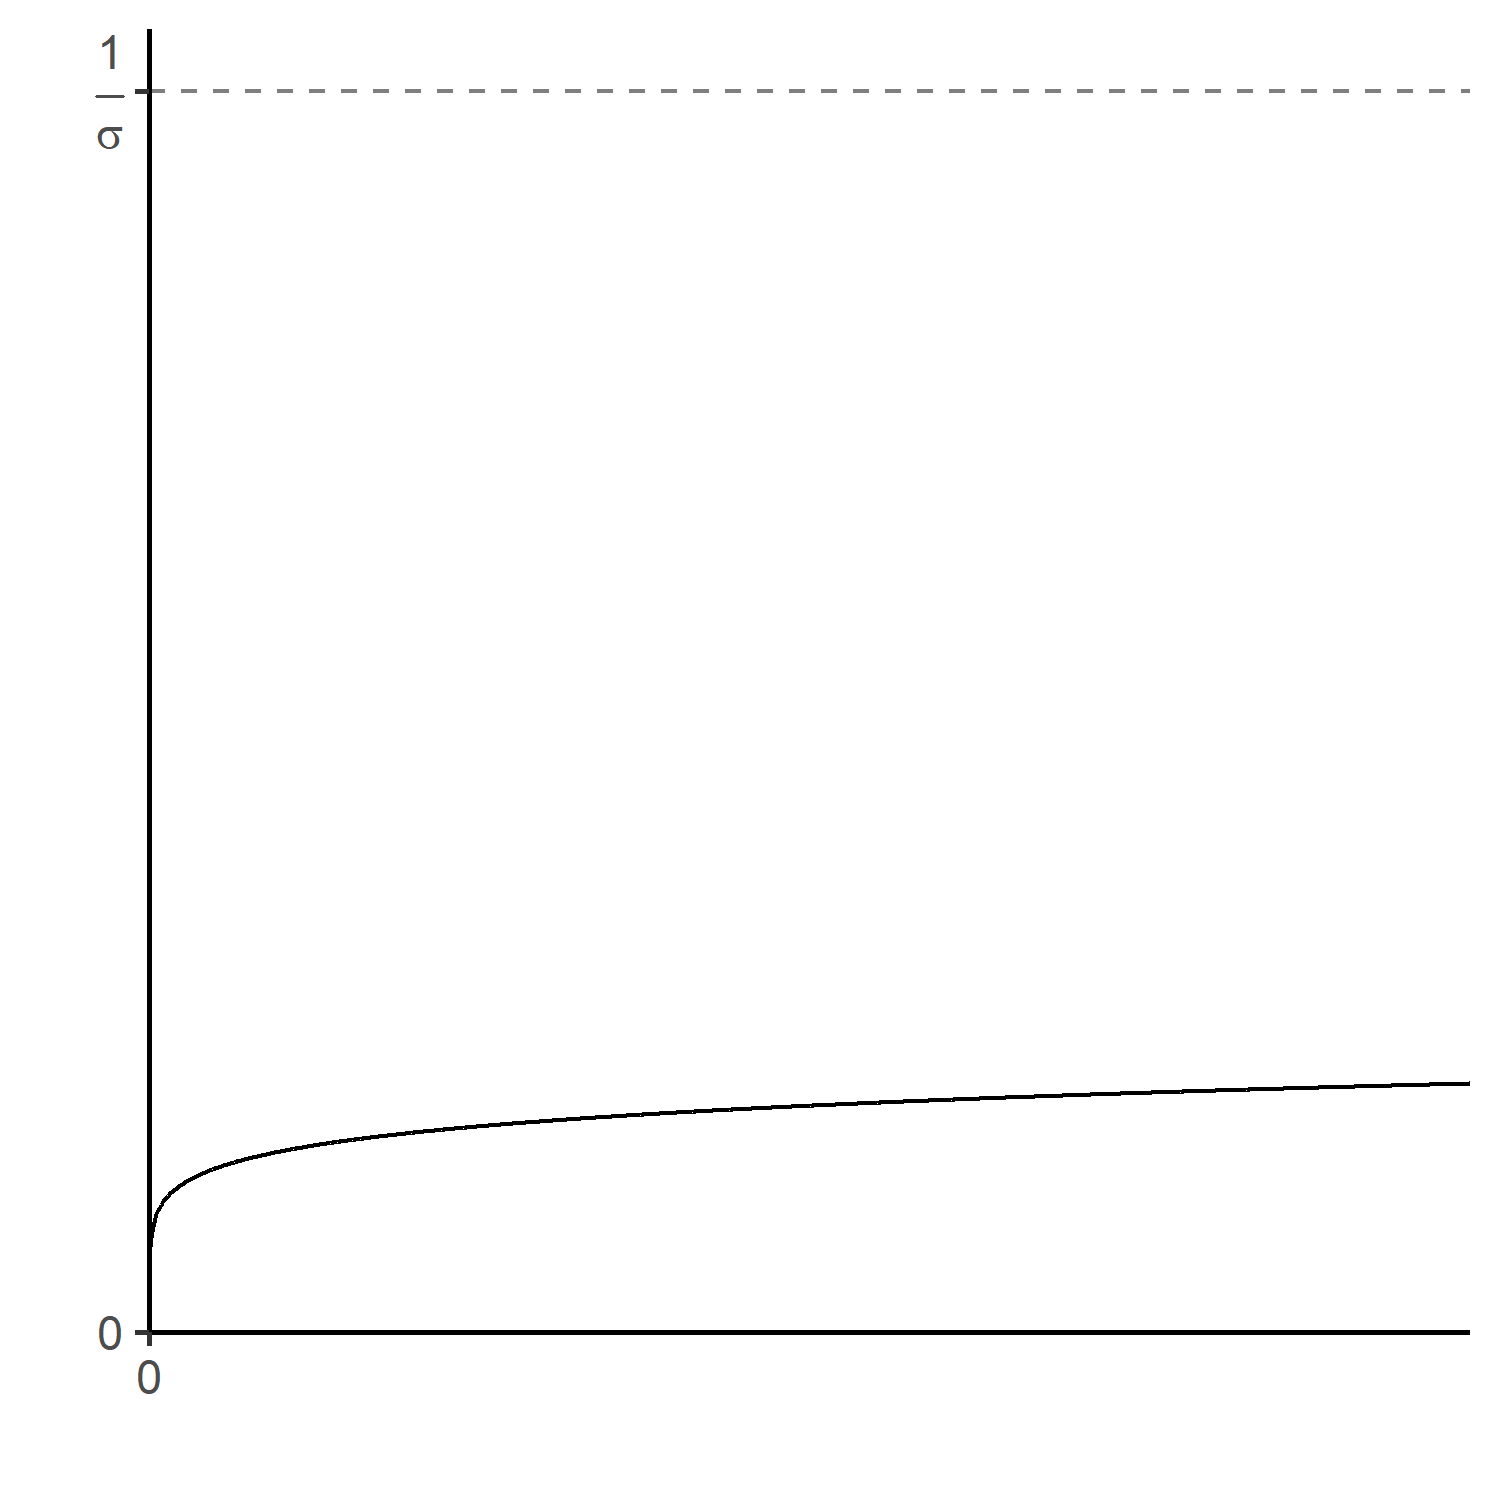
\includegraphics[width=1\linewidth]{../result/appendix_A/function_h/graph_3.png} 
		\caption{$\sigma > 1$} 
		\label{fig:h_shape_3} 
	\end{subfigure} 
	\caption{Different possible shapes of the $h$ function, according to the value of $\sigma$.}
	\label{fig:h_shape}
	\vspace{.5ex}
	\hrule
	\vspace{-4ex}
	\justify\singlespacing\footnotesize The x-axis corresponds to $k_t$. Scales are different according to the graph. The functions graphs are drawn using numerical computation with following set of parameters for each case:\\
	(a) $\sigma = 0.25$, $\phi = 0.3$, $\gamma = 0.5$ ; \hspace{4ex}(b) $\sigma = 0.8$, $\phi = 0.3$, $\gamma = 0.5$ ; \hspace{4ex}(c) $\sigma = 1.2$, $\phi = 0.3$, $\gamma = 0.5$.
\end{figure}

\begin{proposition}\label{prop:full_emp}
	If $k_t \leq k_1$ at the equilibrium, then:
	\begin{enumerate}[label=(\roman*)]
		\item there is a unique equilibrium with full employment where $k_t = k_1$,
		\item the net wage equals the unemployment benefits, i.e. $(1-\tau_t)w_t = b_t$.
	\end{enumerate} 
\end{proposition}
\begin{proof}
	The numerator of the $g$ function is positive if and only if $k_t > k_1 \Leftrightarrow L_t < N_t^y$ (i.e. the number of worker is smaller than the young population size). This condition is always satisfied when there is unemployment. However, if this condition is not satisfied, it would mean that the labor demand exceeds the labor force (i.e. $L_t^d > N_t^y$). Therefore, the economy should face full-employment (i.e. $L_t = N_t^y$) and the capital-per-worker at the equilibrium with full-employment is $k_t = k_1$. In such a case, $X_t$ would tend to  $-\infty$. However, the lower bound of $X_t$ is $0$. Because if $X_t$ is negative, the unemployment benefits would exceed the net wage. I consider that such a case is not possible.\footnote{Even though I consider a model with inelastic labor supply, no agent would work for a wage which is lower than unemployment benefits. This assumption can be considered as an incentive constraint.} Thus, if $k_t \leq k_1 \implies k_t = k_1 \implies u_t = 0 \implies X_t = 0 \implies (1-\tau_t)w_t = b_t$.
\end{proof}

Therefore, the equilibrium with unemployment requires $k_t > k_1$. Hence, any equilibrium in the case represented in figure \ref{fig:g_shape_b} leads to the equilibrium with full-employment.

I normalize $k_t$ to the vertical asymptote $k_1$. Let $\nu = k_2/k_1$ with $\nu > 0$. It implies that $k_2 \gtreqqless k_1$ when $\nu \gtreqqless 1$. Let $\tilde{k}_t = k_t / k_1$ with $\tilde{k}_t > 0$. As for $\nu$, if $\tilde{k}_t$ is greater than unity, then $k_t>k_1$ and vice-versa. To simplify the notation, let $\rho = \frac{\sigma-1}{\sigma} \in \left(-\infty, 1\right)$.\footnote{When both input factors are gross complement, the elasticity of substitution is $\sigma \in \left(0,1\right)$ and the corresponding interval for $\rho$ is $\left(-\infty, 0\right)$. However, when both are gross substitute, the elasticity of substitution is $\sigma \in \left(0,+\infty\right)$ and the corresponding interval for $\rho$ is $\left(0,1\right)$.} Using this specification, it is possible to rewrite $g$ such that:
\begin{equation*}
g(\tilde{k}_t; \nu, \rho) = \ln\left(\frac{\tilde{k}_t - 1}{\tilde{k}_t^\rho - \nu^\rho}\right) + \rho\ln\left(\nu\right)
\end{equation*}
Let also rewrite the $h$ function such that:
\begin{equation*}
h(\tilde{k}_t ; \tilde{\gamma}, \rho) = \left( \frac{1}{1-\rho} + \tilde{\gamma} \tilde{k}_t^{-\rho} \right)^{-1}
\end{equation*}
where $\tilde{\gamma} \equiv \frac{1-\phi}{\phi} \frac{1-\gamma(1-\sigma)}{\gamma} k_1^{-\rho}> 0$.

\subsection*{A.1 Under gross-complementarity, i.e. $\rho < 0$}

$g(\tilde{k}_t)$ is define and continuous between both vertical asymptotes within the logarithm, so $1$ and $\nu$.\footnote{These vertical asymptotes correspond to $k_1$ and $k_2$ before the normalization.} When $\nu$ is greater than unity, $g(\tilde{k}_t)$ is defined and continuous on $\left(1, \nu\right)$. While the function is defined and continuous on $\left(\nu, 1\right)$ when $\nu < 1$. Finally, when $\nu = 1$, $\tilde{k}_t$ can take a unique value which corresponds to $1$. This definition domain is due to the properties of the logarithm. Both parts of the product within the logarithm must have the same sign in order to remain defined. The $g$ function has two possible shapes according to the value of $\nu$ with respect to unity:
\begin{enumerate}
	\item if $\nu > 1$:
	\begin{enumerate}
		\item $g(\tilde{k}_t)$ is strictly increasing in $\tilde{k}_t$,% i.e. $\frac{\partial g}{\partial \tilde{k}_t} > 0$,
		\item $\lim_{\tilde{k}_t\to 1} g(\tilde{k}_t) = -\infty$  and $\lim_{\tilde{k}_t\to \nu} g(\tilde{k}_t) = +\infty$.
	\end{enumerate}
	\item if $\nu < 1$:
	\begin{enumerate}
		\item $g(\tilde{k}_t)$ is strictly decreasing in $\tilde{k}_t$,% i.e. $\frac{\partial g}{\partial \tilde{k}_t} < 0$,
		\item $\lim_{\tilde{k}_t\to 1} g(\tilde{k}_t) = +\infty$ and $\lim_{\tilde{k}_t\to \nu} g(\tilde{k}_t) = -\infty$.
	\end{enumerate}
\end{enumerate}
When $\rho<0$, the $h$ function is defined and continuous on $\mathbb{R}_+$ and has the following properties:
\begin{enumerate}
	\item $h(\tilde{k}_t)$ is strictly decreasing in $\tilde{k}_t$,% i.e. $\frac{\partial h}{\partial \tilde{k}_t} \leq 0$,
	\item $\lim_{\tilde{k}_t\to 0} h(\tilde{k}_t) = 1-\rho$ and $\lim_{\tilde{k}_t\to +\infty} h(\tilde{k}_t) = 0$.
\end{enumerate}

These properties leads to lemmas \ref{lemma:rho_lower0_nu_lower1} and \ref{lemma:rho_lower0_nu_higher1}. Using these intermediate results with proposition \ref{prop:full_emp}, I can prove proposition \ref{prop:full_emp}.
\begin{lemma}\label{lemma:rho_lower0_nu_lower1}
	if $\rho < 0$ and $\nu > 1$, then it exists a unique equilibrium.
\end{lemma}
\begin{proof}
	Let $\rho < 0$ and $\nu > 1$. The $g$ function is defined and continuous in $\tilde{k}_t \in \left(1, \nu \right)$, strictly increasing and has two infinite vertical asymptotes of opposite signs. The $h$ function is defined and continuous in $\tilde{k}_t \in \mathbb{R}_+ \supset \left(1, \nu \right)$, strictly decreasing and has two finite horizontal asymptotes $1/\sigma$ and $0$. Therefore, both functions intersect in only one point. Hence, there is uniqueness of the equilibrium.
\end{proof}
\begin{lemma}\label{lemma:rho_lower0_nu_higher1}
	if $\rho < 0$ and $\nu < 1$, then it exists at least one equilibrium.
\end{lemma}
\begin{proof}
	Let $\rho < 0$ and $\nu > 1$. The $g$ function is defined and continuous in $\tilde{k}_t \in \left(\nu, 1\right)$, strictly decreasing and has two infinite vertical asymptotes of opposite signs. The $h$ function is defined and continuous in $\tilde{k}_t \in \mathbb{R}_+ \supset \left(\nu, 1\right)$, strictly decreasing and has two finite horizontal asymptotes $1-\rho$ and $0$. Therefore, both functions intersect in at least one point. Hence, there is at least one equilibrium.
\end{proof}
\begin{proposition}
	if $\rho < 0$, then it exists a unique equilibrium.
\end{proposition}
\begin{proof}
	Lemma \ref{lemma:rho_lower0_nu_lower1} claims that there is a unique equilibrium when $\nu > 1$. There is also a unique equilibrium when $\nu = 1$. Lemma \ref{lemma:rho_lower0_nu_higher1} asserts that there is at least one equilibrium when $\nu < 1$. Yet, proposition \ref{prop:full_emp} states that any equilibrium when $\nu > 1$ leads to the unique equilibrium with full-employment. Therefore, if $\rho < 0$ there is a unique equilibrium.
\end{proof}

\subsection*{A.2 Under gross-substituability, i.e $0 < \rho < 1$}

Contrary to the previous case, $g(\tilde{k}_t)$ is defined and continuous on $\mathbb{R}_+$ but outside of both vertical asymptotes within the logarithm, so $1$ and $\nu$. When $\nu$ is greater than unity, $g(\tilde{k}_t)$ is defined and continuous on $(0, 1) \cap (\nu, +\infty)$. While the function is defined and continuous on $(0, \nu) \cap (1, +\infty)$ when $\nu < 1$. Finally, when $\nu = 1$, the function is defined and continuous on $\mathbb{R}_+$ but has no longer infinite discontinuity. Regardless of the value of $\nu$, $\lim_{\tilde{k}_t\to 0} = 0$ and $\lim_{\tilde{k}_t\to +\infty} = +\infty$. Both vertical asymptotes correspond to $\lim_{\tilde{k}_t\to 1} g(\tilde{k}_t) = -\infty$ and $\lim_{\tilde{k}_t\to \nu} g(\tilde{k}_t) = +\infty$. The $g$ function has two possible shapes according to the value of $\nu$ with respect to unity.\footnote{Excluding the case where $\nu=1$.} Moreover, $g(\tilde{k}_t)$ is strictly increasing in $\tilde{k}_t$ when $\nu < 1$. When $\rho > 1$, the $h$ function is defined and continuous on $\mathbb{R}_+$ and has the following properties:
\begin{enumerate}
	\item $h(\tilde{k}_t)$ is strictly increasing in $\tilde{k}_t$,
	\item $\lim_{\tilde{k}_t\to 0} h(\tilde{k}_t) = 0$ and $\lim_{\tilde{k}_t\to +\infty} h(\tilde{k}_t) = 1-\rho$.
\end{enumerate}
I plot both functions with numerical computation for feasible values of $\sigma$ according to the model conditions as detailed in section \ref{subsec:wage_bargaining}. The parameters $\gamma$ and $\phi$ are set according to the calibration in section \ref{subsec:calibration}, thus $\gamma = 0.5$ and $\phi = 0.3$.\footnote{The exact values for $\phi$ are 0.27 for France and 0.325 for the United-States. I use 0.3 for this numerical computation as an approximation of the mean.} Figure \ref{fig:gh2} shows both functions in the case where $\nu < 1$.
\begin{figure}[tb]
	\centering
	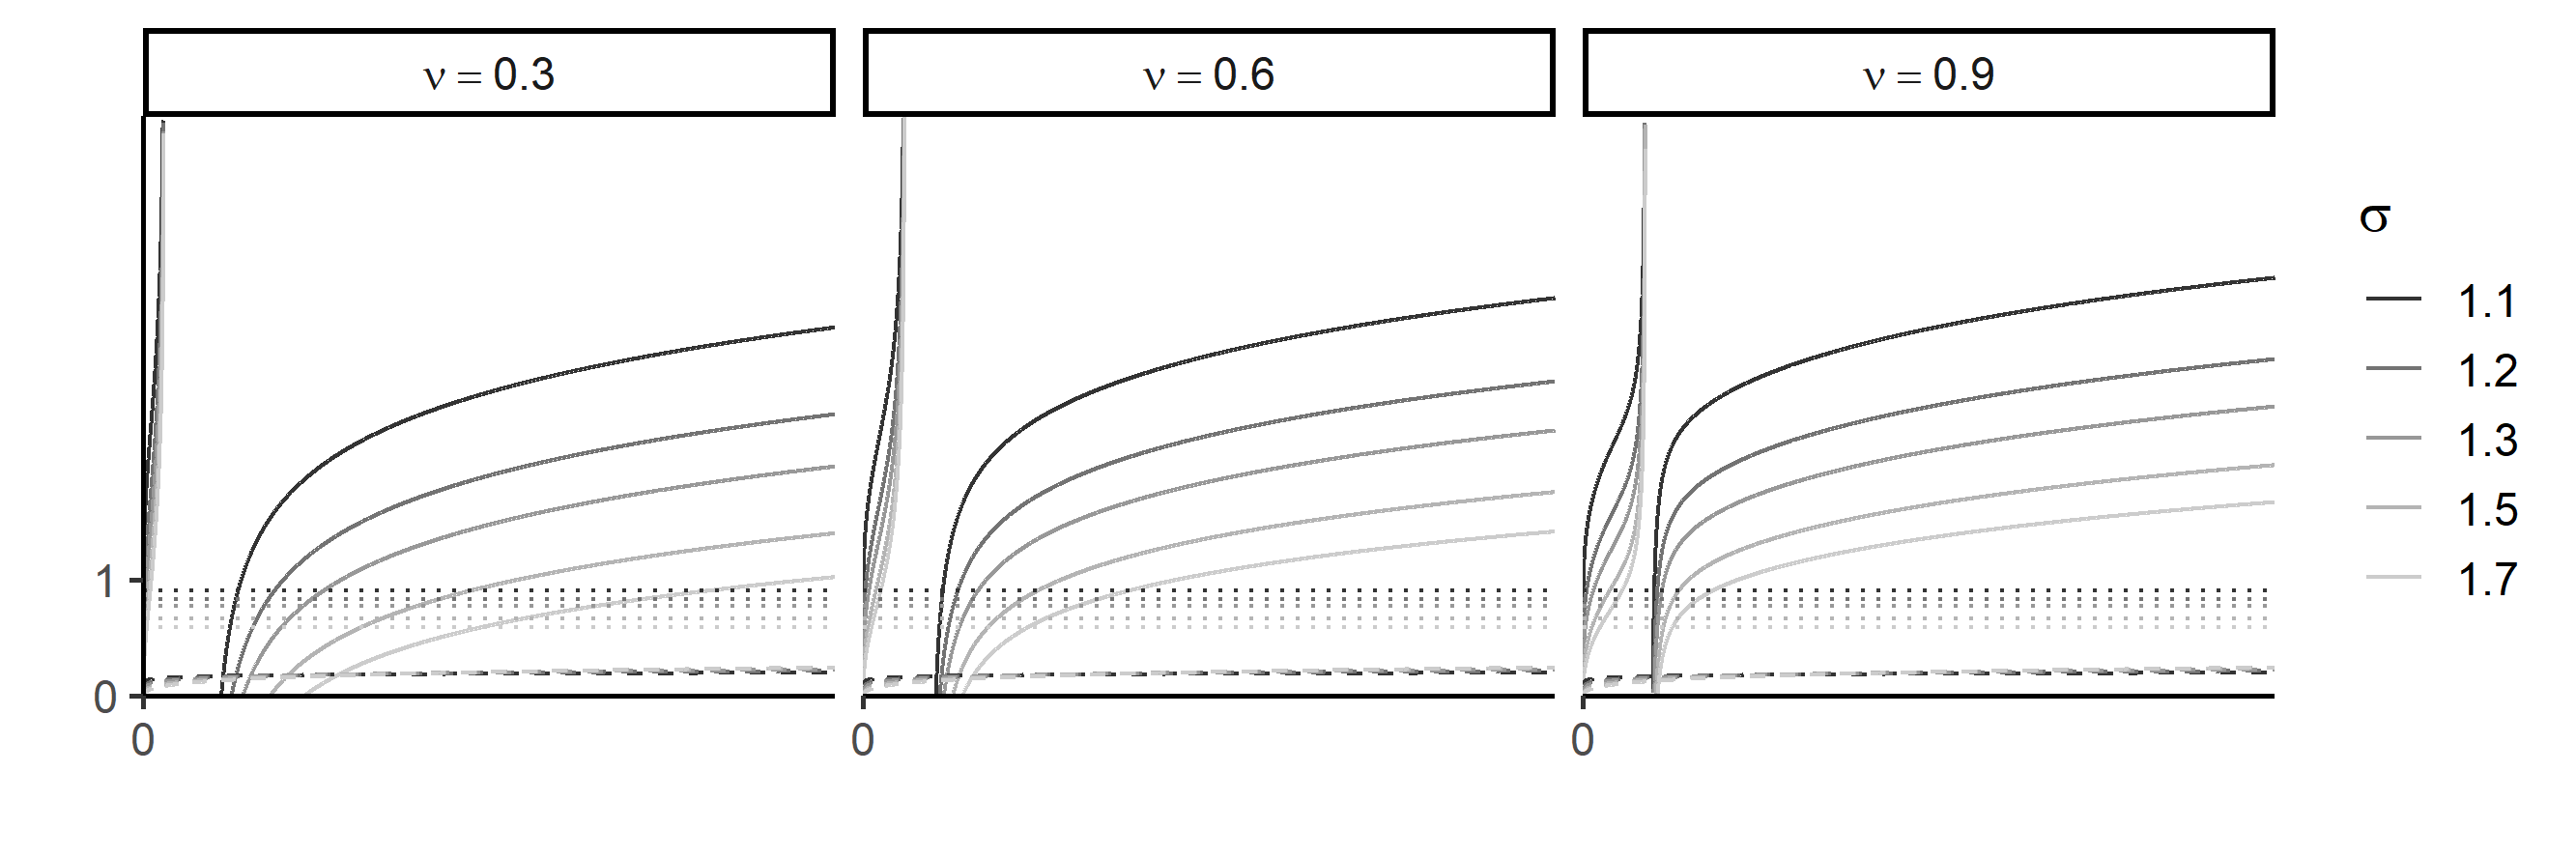
\includegraphics[width = 1\linewidth]{../result/appendix_A/uniqueness/gd_all.png}
	\caption{Numerical simulation of $g$ (solid line) and $h$ (dashed line), according to the values of $\sigma$ and $\nu$.}
	\label{fig:gh2}
	\vspace{.5ex}
	\hrule
	\vspace{-4ex}
	\justify\singlespacing\footnotesize The x-axis corresponds to $\tilde{k}_t$. The dotted lines correspond to $1-\rho$, so the infinite limit in $\tilde{k}_t$ of the $h$ function.
\end{figure}
Looking at the behavior of both functions, they do intersect in only one point beyond $1$. Therefore, I make the following conjecture:
\begin{conjecture}\label{conj:rho_higher0_nu_lower1}
	if $\rho \in (0,1)$ and $\nu < 1$, then it exists a unique equilibrium.
\end{conjecture}
This unique equilibrium is the one with unemployment since it lies beyond $1$ and therefore beyond $k_1$ without normalization. I also do the numerical computation in the case where $\nu > 1$, with the same values for $\gamma$ and $\phi$. Figure \ref{fig:gh1} plots the result.
\begin{figure}[tb]
	\centering
	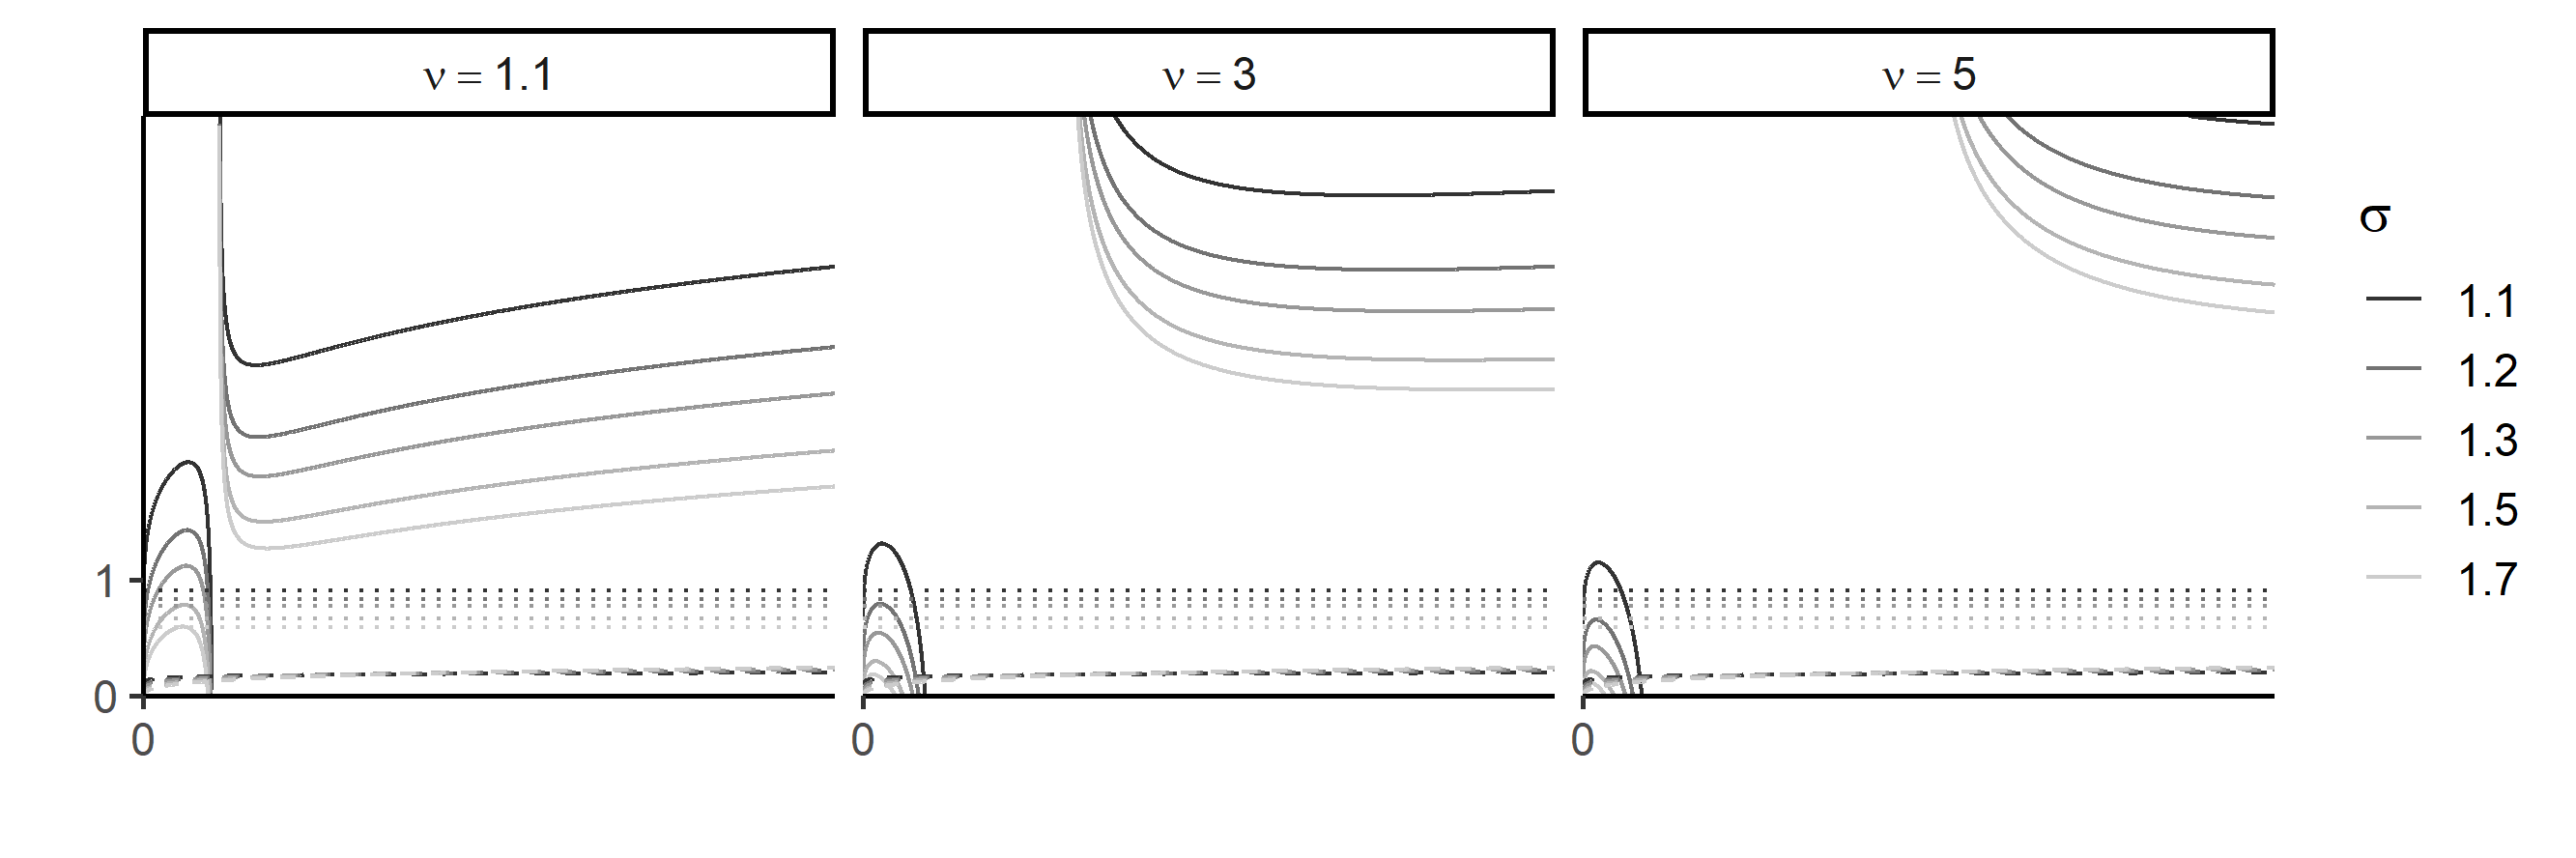
\includegraphics[width = 1\linewidth]{../result/appendix_A/uniqueness/gc_all.png}
	\caption{Numerical simulation of $g$ (solid line) and $h$ (dashed line), according to the values of $\sigma$ and $\nu$.}
	\label{fig:gh1}
	\vspace{.5ex}
	\hrule
	\vspace{-4ex}
	\justify\singlespacing\footnotesize The x-axis corresponds to $\tilde{k}_t$. The dotted lines correspond to $1-\rho$, so the infinite limit in $\tilde{k}_t$ of the $h$ function.
\end{figure}
Looking at the behavior of both functions, they do intersect two times before $1$. Therefore, I make the following conjecture:
\begin{conjecture}\label{conj:rho_higher0_nu_higher1}
	if $\rho \in (0,1)$ and $\nu > 1$, then it exists at least one equilibrium lying below unity.
\end{conjecture}
Using these two conjectures with proposition \ref{prop:full_emp}, I can prove that there is a unique equilibrium for all $\rho \in (0,1)$.\footnote{Except in the case where $\nu = 1$, i.e. $k_1 = k_2$. In such a case, the infinite discontinuity disappears and so does the equilibrium.}
\begin{proposition}
	if $\rho \in (0,1)$, then it exists a unique equilibrium.
\end{proposition}
\begin{proof}
	Conjecture \ref{conj:rho_higher0_nu_lower1} claims that there is a unique equilibrium when $\nu < 1$. Conjecture \ref{conj:rho_higher0_nu_higher1} asserts that there is at least one equilibrium when $\nu > 1$ lying below unity. Thus, there is at least one equilibrium such that $k_t < k_1$. Yet, proposition \ref{prop:full_emp} states that any equilibrium with $k_t \leq k_1$ leads to the unique equilibrium with full-employment. Therefore, if $\rho \in (0,1)$ there is a unique equilibrium.
\end{proof}



